\chapter{Agujeros Negros ***PRELIMINAR***}


\section{Singularidades y radio de Schwarzschild}

Aqu'i estudiaremos la estructura de la soluci'on de Schwarzschild en regiones \textit{cercanas al radio de Schwarzschild}, donde el campo gravitacional es muy intenso. En otras palabras, estudiaremos las geometr'ia del espaciotiempo esf'ericamente sim'etrico de una masa $M$ suficientemente compacta para que su tama\~no (la coordenada radial correspondiente a su superficie) sea menor que $2m$. Por ahora, postergaremos la importante discusi'on acerca de si existe un mecanismo f'isico realista para que una distribuci'on de masa pueda llegar a esta configuraci'on.

La geometr'ia del espaciotiempo de Schwarzschild, en coordenadas de
curvatura, es decir (\ref{Sch}), parece tener un mal comportamiento cerca de
$r=0$ y adem'as en $r=2m$, es decir, en el origen y en la esfera definida por
la condici'on que la coordenada radial $r$ sea igual al radio de Schwarzschild.
\begin{eqnarray}
 g_{00}&\to& -\infty,\quad g_{11}\to 0, \qquad \text{para}\quad r\to 0 ,\\
 g_{00}&\to& 0,\quad g_{11}\to -\infty, \qquad \text{para}\quad r\to 2m^+ .
\end{eqnarray}
Los coeficientes m'etricos son cantidades dependientes de las coordenadas
usadas, por lo que sus valores no necesariamente est'an relacionados con
cantidades f'isicas singulares. Para saber si estos comportamientos
singulares/divergentes son f'isicos, o s'olo \textit{singularidades coordenadas},
necesitamos considerar propiedades que sean independientes de las coordenadas
usadas.

Es relativamente f'acil generar singularidades coordenadas. Consideremos por ejemplo, el espacio euclidiano bidimensional $E_2$, con su elemento de l'inea en coordenadas cartesianas:
\begin{equation}
ds^2=dx^2+dy^2.
\end{equation}
Si introducimos una nueva coordenada $\xi$ por medio de
\begin{equation}
\xi:=\frac{1}{3}x^3,
\end{equation}
tendremos que la m'etrica toma la forma%
\begin{equation}
ds^2 =\left( 3\xi\right) ^{-\frac{4}{3}}d\xi^2+dy^2.
\end{equation}
La m'etrica parece tener ahora una singularidad en $\xi=0$. Sin embargo, esta
singularidad es totalmente removible introduciendo una ``nueva"\, variable $x$ por
medio de $\xi=x^3/3$. Por esto, se dice que 'esta es una
\textit{singularidad coordenada}. Es posible que tengamos una singularidad coordenada que sea el resultado de un quiebre de un sistema coordenado espec'ifico en lugar de ser una singularidad de la variedad subyacente. En otras palabras, se dice que la variedad tiene una singularidad (``verdadera'' o ``intr'inseca'') en su geometr'ia \textit{si ella no puede ser removida por un cambio de coordenadas apropiado}. En general no es obvio encontrar la manera de remover una singularidad coordenada.

Una forma de testear si una regi'on contiene singularidades de la geometr'ia (es decir, que no sean simples singularidades coordenadas) es calcular invariantes (es decir, escalares) a partir de contracciones del tensor de curvatura. Los escalares m'as simples son el escalar de curvatura
$R$, y sus contracciones $R_{\mu\nu\rho\sigma}R^{\mu\nu\rho\sigma}$, $R_{\mu\nu\rho\sigma}R^{\rho\sigma\lambda\tau}R^{\mu\nu}{}_{\lambda\tau}$, etc. Si alguno de estos escalares \textit{diverge} al acercarse a alg'un punto, tal punto es una singularidad de la geometr'ia. As'i, tenemos una condici'on \textit{suficiente}
para mostrar que un punto es una singularidad de la geometr'ia. Por otro lado, en general no es f'acil mostrar que un punto \textit{no es} singularidad.

En el caso de la m'etrica de Schwarzschild un c'alculo directo muestra que
\begin{equation}
R_{\mu\nu\rho\sigma}R^{\mu\nu\rho\sigma}=\frac{48m^2}{r^6},
\end{equation}
lo que prueba que $r=0$ (el origen del sistema coordenado usado) representa una
singularidad de la geometr'ia, donde la curvatura diverge. Puede verificarse que en $r=2m$ ninguno de los invariantes de curvatura arriba mencionados diverge. Por lo tanto, la esfera definida por $r=2m$ no es una singularidad de la curvatura (que mide propiedades locales de la variedad), sino algo diferente ...

\begin{itemize}
\item En $r=2m$, $g_{11}$ es infinito y $g_{00}$ es cero. Dado que $g_{00}
$ es cero, la superficie esf'erica en $r=2m$ es una \textit{superficie
infinitamente desplazada al rojo} por efecto de la dilataci'on temporal gravitacional. Ver la expresi'on (\ref{rgsch}). Decimos entonces que la superficie $r=2m$ es una \textit{superficie de redshift infinito}.

\item Adem'as, cuando $r<2m$, el signo de las componentes $g_{00}$ y $g_{11}$ cambian: $g_{00}$ se convierte en negativo y $g_{11}$ en positivo. Esto nos fuerza a reconsiderar el significado f'isico de $t$ y $r$. En efecto, en la regi'on del espaciotiempo con $r<2m$, $t$ es una coordenada tipo espacio y $r$ tipo tiempo, ya que una curva a lo largo del eje $t$ ($r$, $\theta$ y $\varphi$ constantes) posee $ds^2<0$, mientras que una curva a lo largo del eje $r$ ($t$, $\theta$ y $\varphi$ constantes) posee $ds^2>0$. Como veremos m'as adelante, esto trae como consecuencia que toda part'icula dentro de la regi'on delimitada por $r=2m$ caer'a hacia la singularidad central. Debido a esto, la superficie $r=2m$ es adicionalmente un \textit{horizonte de eventos}.
\end{itemize}

Estas caracter'isticas muestran que $r=2m$ es un radio inusual, pero
esto no implica que la geometr'ia local del espaciotiempo sea
singular en $r=2m$, como s'i ocurre en $r=0$.

Para analizar las propiedades f'isicas de la regi'on en torno a $r=2m$ con m'as detalle, estudiaremos las propiedades de fotones y de part'iculas en movimiento radial ``cayendo'' hacia (y ``escapando'' desde) la singularidad central.

\subsection{Diagrama Espacio-Temporal en Coordenadas de Schwarzschild}

Una manera de entender una geometr'ia es explorando su estructura causal, que est'a definida por las propiedades de propagaci'on de la luz. Consideremos en particular curvas (geod'esicas)
radiales tipo luz, es decir, para las cuales $\theta$ y $\varphi$ son constantes y
$ds^2=0$. Esta 'ultima condici'on se reduce a
\begin{equation}
 \left(1-\frac{2m}{r}\right) c^2dt^2-\frac{dr^2}{\left( 1-\frac
{2m}{r}\right) }=0,
\end{equation}
de donde obtenemos que
\begin{equation}
 c\frac{dt}{dr}=\pm\frac{1}{\left| 1-\frac{2m}{r}\right|}. \label{dtdr1}
\end{equation}
Considerando que
\begin{equation}
 \int_a^b\frac{dr}{\left| 1-\frac{2m}{r}\right|}=\pm\left[b-a+2m\ln\left(\frac{b-2m}{a-2m}\right)\right], \quad a<b,
\end{equation}
donde el signo positivo y negativo corresponde a los casos en que $a,b>2m$ y $a,b<2m$, respectivamente, podemos integrar (\ref{dtdr1}).

Si $r>2m$ el signo $+$ en (\ref{dtdr1}) corresponde a fotones alej'andose del centro de simetr'ia y el signo $-$ a fotones acerc'andose a 'este. En este caso obtenemos,
\begin{equation}
 c(t-t_0)=r-r_0+2m\ln\left(\frac{r-2m}{r_0-2m}\right),  \label{rtfs}
\end{equation}
para fotones salientes, y
\begin{equation}
 c(t-t_0)=r_0-r-2m\ln\left(\frac{r-2m}{r_0-2m}\right), \label{rtfe}
\end{equation}
para fotones entrantes, que pasan por el evento con coordenadas $(ct_0,r_0)$, respectivamente.
\begin{figure}[H]
 \begin{center}
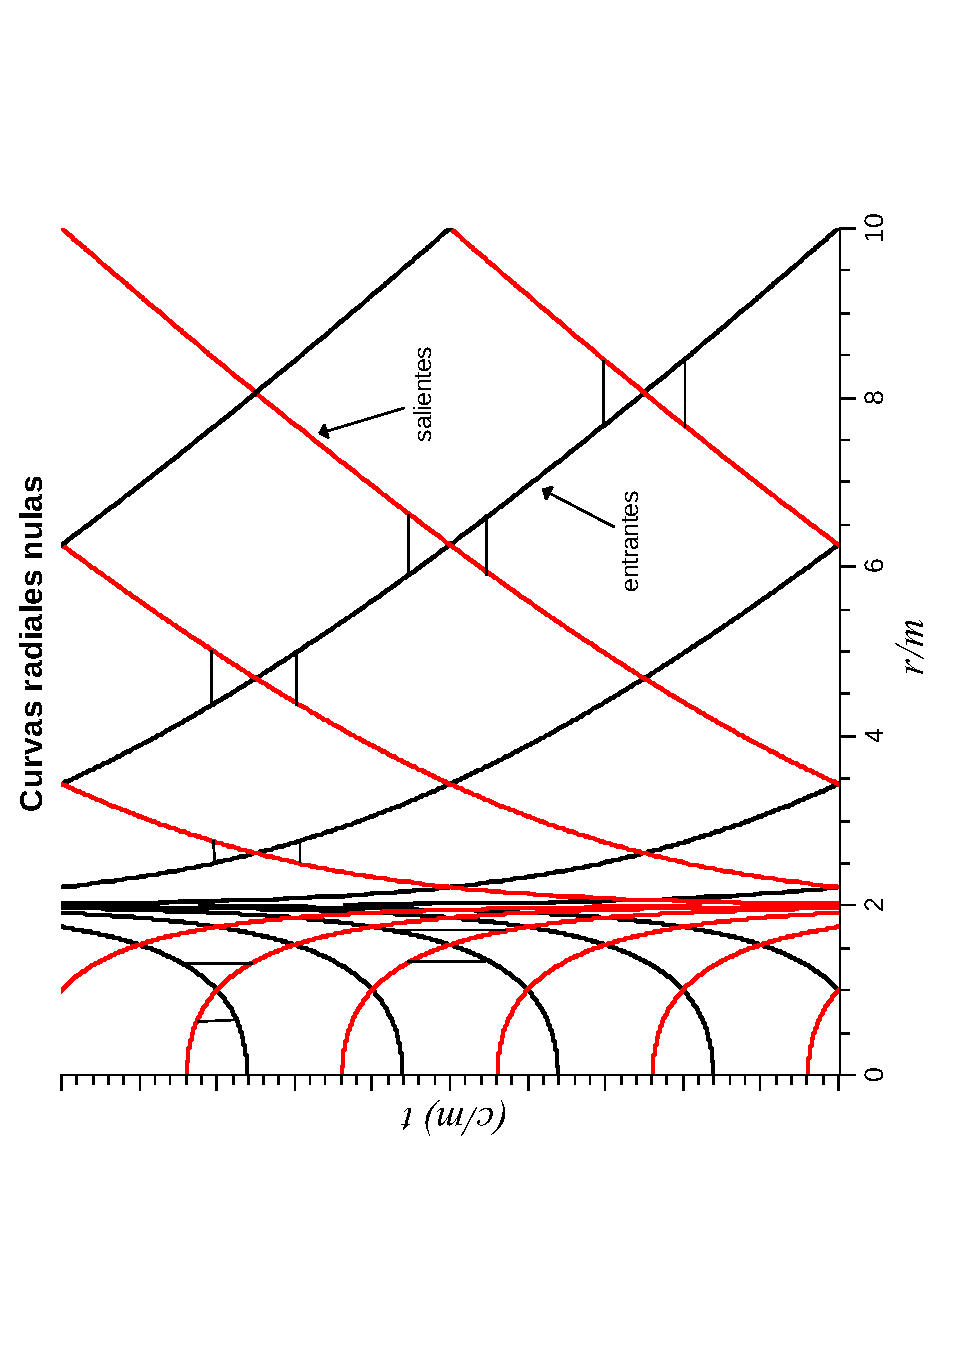
\includegraphics[height=8cm,angle=-90]{fig/fig-nullrays-cc-01.pdf}
\caption{Curvas nulas radiales en coordenadas de curvatura.}
\label{fig:nullrays-cc}
\end{center}
\end{figure}
Como es de esperar, muy lejos del centro de fuerzas $r\gg 2m$, recobramos
\begin{equation}
\frac{dr}{dt}=\pm\, c,
\end{equation}
tal como en un espaciotiempo plano. Por otro lado, cuando $r$ se aproxima a $2m$ (por ``la derecha'', es decir, con valores mayores a $2m$), tenemos
\begin{equation}
\frac{dt}{dr}\rightarrow\pm\infty,
\end{equation}
y los conos de luz se ``cierran", ya que las l'ineas tienden a ser
paralelas al eje $t$. Esto tendr'a como consecuencia que al acercarse a $r=2m$ la coordenada temporal de la trayectoria del fot'on aumentar'a indefinidamente. En otras palabras, en t'erminos de la coordenada temporal $t$, a medida que un rayo de luz se aproxima a $r=2m$ pareciera que el fot'on nunca llegar'a all'i. En realidad, como veremos a continuaci'on, un rayo de luz no tiene problemas en alcanzar $r=2m$ (tampoco part'iculas masivas), pero un observador lejos de $r=2m$ nunca ser'ia capaz de ``ver'' este hecho.

En efecto, para describir c'omo se ``ve''\, la ca'ida del fot'on desde lejos, consideraremos un observador en reposo en $r=R>2m$ y c'omo 'este puede informarse sobre la ca'ida del fot'on.

Para esto, consideramos un fot'on cayendo hacia la singularidad, y dos eventos $E_1$ y $E_2$ en su l'inea de mundo, con coordenadas $(ct,r)=(ct_1,r_1)$ y $(ct,r)=(ct_2,r_2)$ respectivamente, con $r_2<r_1<R$. De acuerdo a lo anterior, las coordenadas de estos eventos est'an relacionadas por medio de
\begin{equation}
c(t_2-t_1)=r_1-r_2+2m\ln\left(\frac{r_1-2m}{r_2-2m}\right). \label{t2t1}
\end{equation}
Consideremos que cuando el fot'on pasa por el evento $E_1$ una se~nal luminosa (otro fot'on) es enviada hacia el observador en $R>r_1$. Este nuevo fot'on viaja desde el evento $E_1$ hasta el evento de recepci'on $R_1$, con coordenadas $(ct,r)=(ct_{1\rm r},R)$. Como estos eventos pertenecen a la l'inea de mundo de un fot'on alej'andose de la singularidad, sus coordenadas satisfacen
\begin{equation}
c(t_{1 \rm r}-t_1)=R-r_1+2m\ln\left(\frac{R-2m}{r_1-2m}\right).\label{t1rt1}
\end{equation}
Similarmente, si en el evento $E_2$ se emite una segunda se\~nal luminosa hasta el observador, de modo que 'este la recibe en el evento $R_2$ con coordenadas $(ct,r)=(ct_{2\rm r},R)$, entonces
\begin{equation}
c(t_{2 \rm r}-t_2)=R-r_2+2m\ln\left(\frac{R-2m}{r_2-2m}\right).\label{t2rt2}
\end{equation}
El intervalo de coordenada temporal entre la recepci'on de las dos se~nales por el observador en reposo en la posici'on $r=R$ es dada por $(\Delta t)_{\rm r}=t_{2 \rm r}-t_{1 \rm r}$. Usando (\ref{t2t1}), (\ref{t1rt1}) y (\ref{t2rt2}), encontramos
\begin{equation}
c(\Delta t)_{\rm r}=2\left[r_1-r_2+2m\ln\left(\frac{r_1-2m}{r_2-2m}\right)\right].
\end{equation}
En otras palabras, $(\Delta t)_{\rm r}=2(t_2-t_1)$. Finalmente, el tiempo (propio) medido por el observador en $r=R$ entre las dos se~nales es $(\Delta\tau)_{\rm r}=(\Delta t)_{\rm r}\sqrt{1-2m/R}$. En particular, para un observador ``en el infinito", tendremos simplemente que
$(\Delta\tau)_{{\rm r},\infty}=2(t_2-t_1)$. Como consecuencia, desde el punto de vista de un observador externo (en $r=R$, o en el infinito) el fot'on requiere un tiempo infinito en llegar a $r=2m$, es decir, \textit{el observador nunca registra que el fot'on cruza el horizonte}, sino que lo observa acercarse cada vez m'as lentamente. No obtante, como veremos a continuaci'on, el fot'on no encuentra ning'un obst'aculo al acercarse al horizonte, cruz'andolo y alcanzando finalmente la singularidad central.

\subsection{Coordenadas de Eddington-Finkelstein}

Hemos visto que en t'erminos de las coordenadas de curvatura los conos de luz parecen comprimirse a medida que se acercan a $r=2m$, y que las curvas tipo luz radiales entrantes parecen nunca cruzar el horizonte, ya que estas curvas se tornan cada vez m'as verticales.

Es posible introducir nuevas coordenadas en las que estas caracter'isticas no est'an presentes. Espec'ificamente, podemos elegir nuevas coordenadas $\bar{x}^\mu=(c\bar{t},r,\theta,\varphi)$, en las que las l'ineas nulas radiales entrantes sean rectas con un 'angulo de 45 grados respecto al eje $r$. De (\ref{rtfe}) vemos que si definimos la \textit{coordenada de Eddington-Finkelstein retardada} por
\begin{equation}
 \bar{t}(t,r):=t+\frac{2m}{c}\ln\left|r-2m\right|, \label{tEF}
\end{equation}
entonces la relaci'on que define la trayectoria de un fot'on entrante es simplemente
\begin{equation}
 c(\bar{t}-\bar{t}_0)=r_0-r,
\end{equation}
que en el plano $(c\bar{t},r)$  corresponde precisamente una l'inea recta con pendiente $-1$.

En t'erminos de las nuevas coordenadas $\bar{x}^\mu$ el elemento de l'inea adopta la forma siguiente:
\begin{equation}\marginnote{Schwarzschild, Eddington-Finkelstein}
 ds^2=\left(1-\frac{2m}{r}\right)c^2d\bar{t}^2-\frac{4m}{r}c\,d\bar{t}\,dr-\left(1+\frac{2m}{r}\right)dr^2-r^2\left(d\theta^2+\sen^2\theta\,d\varphi^2\right). \label{dsEF}
\end{equation}
Vemos que la m'etrica en estas coordenadas es regular en $r=2m$. De hecho, ella es regular en todo el rango $0<r<2m$. Puede argumentarse que la transformaci'on (\ref{tEF}) no es v'alida para puntos con $r\le 2m$ y que por consiguiente (\ref{dsEF}) s'olo ser'ia v'alida en la regi'on fuera del horizonte. Sin embargo, en la teor'ia de RG, la m'etrica de Schwarzschild en coordenadas de curvatura, con $0<r<\infty$ es una soluci'on tan leg'itima de las ecuaciones de Einstein en el vac'io como lo es la m'etrica asociada a (\ref{dsEF}) con $0<r<\infty$. En general, el criterio usado es que, dada una m'etrica que es soluci'on de las Ecuaciones de Einstein, se busca el rango m'aximo de variaci'on de las coordenadas tales que la soluci'on sea v'alida. En otras palabras, puede perfectamente considerarse la m'etrica en coordenadas de Eddington-Finkelstein como la ``m'etrica original'', v'alida en todo el rango $0<r<\infty$, y la m'etrica en coordenadas de curvatura como s'olo apropiada en la regi'on exterior al horizonte. En cierto sentido, la m'etrica en coordenadas Eddington-Finkelstein es una suerte de ``continuaci'on anal'itica'' de la m'etrica de la soluci'on en coordenadas de curvatura.

Como vimos, en coordenadas de Eddington-Finkelstein, las l'ineas nulas radiales entrantes son l'ineas rectas. Por otro lado, las curvas nulas radiales \textit{salientes} est'an descritas por la relaci'on
\begin{equation}
 c(\bar{t}-\bar{t}_0)=r-r_0+4m\ln\left|\frac{r-2m}{r_0-2m}\right|,  \label{rtfsEF}
\end{equation}
que se obtiene directamente de (\ref{rtfs}) y la definici'on (\ref{tEF}).

\begin{figure}[H]
 \begin{center}
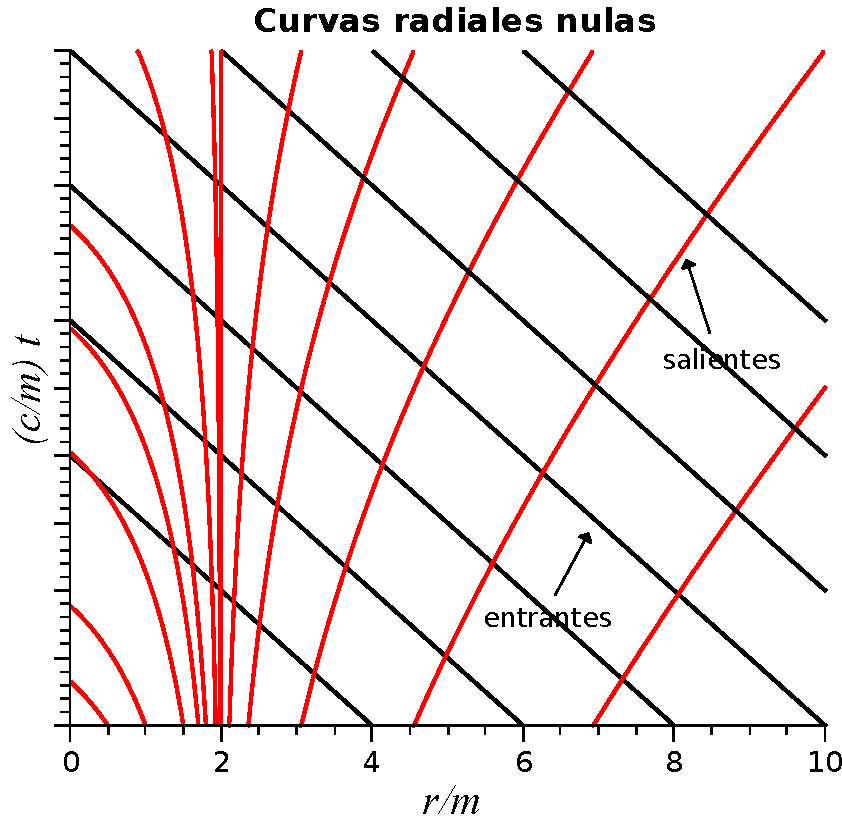
\includegraphics[height=6cm]{fig/fig-nullrays-cEF-2.pdf}
\caption{Curvas nulas radiales en coordenadas de Eddington-Finkelstein.}
\label{fig:nullrays-cEF}
\end{center}
\end{figure}

Vemos que la superficie definida por $r=2m$ act'ua como una ``membrana unidireccional'', en el sentido que s'olo permite cruzar a part'iculas cayendo hacia la singularidad central. Las l'ineas de mundo entrantes cruzan desde la regi'on externa hacia la interna. La superficie $r=2m$ es llamada un \textit{horizonte de eventos} ya que representa la regi'on que delimita los eventos que pueden ser en principio observados por un observador externo. El horizonte de Schwarzschild es \textit{absoluto} en el sentido que impide \textit{a todo observador externo} obtener informaci'on de eventos dentro del horizonte.

\subsection{Part'iculas cayendo radialmente}

Consideremos la trayectoria de una part'icula cayendo libremente en un movimiento radial hacia la singularidad. La trayectoria es entonces una geod'esica radial tipo tiempo. De acuerdo a lo estudiado anteriormente, en este caso la trayectoria tiene como constantes de movimiento a $k$ y $h$ dadas por (\ref{kh}), con $h=0$. De entre las posibles trayectorias, deteminadas por la constante $k$, nos concentraremos en aquellas correspondientes a part'iculas que caen  ``desde el reposo en el infinito'', es decir, tal que $\dot{r}\to 0$ para $r\to\infty$. En este caso la relaci'on (\ref{uuc22}) implica que $k^2=1$. Finalmente, (\ref{kh}a), muestra que para trayectorias ``orientadas hacia el futuro'', $k=1$. Con esto, (\ref{uuc22}) se reduce en este caso a
\begin{equation}
\dot{r}^2 =\frac{2mc^2}{r} .\label{pi1}
\end{equation}
Como estamos considerando una part'icula acerc'andose a la singularidad central, tendremos entonces que
\begin{equation}
\frac{dr}{d\tau}=-c\sqrt{\frac{2m}{r}} .
\end{equation}
Podemos integrar esta expresi'on directamente, y obtenemos
\begin{equation}
 c(\tau-\tau_0)=\frac{2}{3\sqrt{2m}}\left(r_0^{3/2}-r^{3/2}\right), \label{taurclr}
\end{equation}
donde $\tau_0$ es el tiempo propio (del reloj com'ovil con la part'icula) registrado en el instante en que 'esta pasa por $r=r_0$. Note que la expresi'on encontrada, (\ref{taurclr}), es la misma que el caso newtoniano. Como consecuencia, el intervalo de tiempo propio desde que la part'icula cruza $r=r_0$ y que llega a la singularidad central es finito:
\begin{equation}
 c(\tau|_{r=0}-\tau_0)=\frac{2}{3\sqrt{2m}}r_0^{3/2}.
\end{equation}
En particular, el tiempo propio requerido para caer desde el horizonte hasta la singularidad central es $4m/3c$

Para analizar c'omo var'ia la coordenada $t$ en este proceso, podemos escribir
\begin{equation}
 c\frac{dt}{dr}=c\frac{\dot{t}}{\dot{r}}=-\frac{1}{1-\frac{2m}{r}}\sqrt{\frac{r}{2m}}.
\end{equation}
Integrando esta expresi'on\footnote{$\int\sqrt{\frac{r}{a}}\frac{dr}{1-\frac{a}{r}}=\frac{2}{3}a\, (r/a)^{3/2}+2a\,(r/a)^{1/2}-a\ln\left(\frac{\sqrt{r}-\sqrt{a}}{\sqrt{r}+\sqrt{a}}\right) $.} encontramos
\begin{equation}
c(t-t_0)=-\frac{2}{3\sqrt{2m}}\left(r^{3/2} -r_0^{3/2}+6m\sqrt{r}-6m\sqrt{r_0}\right)+2m\ln\left[\frac{(\sqrt{r}+\sqrt{2m})(\sqrt{r_0}-\sqrt{2m})}{(\sqrt{r}-\sqrt{2m})(\sqrt{r_0}+\sqrt{2m})}\right].
\end{equation}
Vemos de esta expresi'on que la coordenada temporal de la trayectoria de la part'icula crece indefinidamente a medida que 'esta se acerca al horizonte.

% \section{Coordenadas de Eddington-Finkelstein}
%
% \begin{align}
% \left[ \left( 1-\frac{2m}{r}\right) \frac{2m^2}{\left(
% r-2m\right) ^2}-\frac{1}{\left( 1-\frac{2m}{r}\right) }\right]
% dr^2 & =\left[ \frac{2m^2}{r\left( r-2m\right) }-\frac
% {1}{\left( 1-\frac{2m}{r}\right) }\right] dr^2\\
% & =\left[ \frac{\left( 1-\frac{2m}{r}\right) 2m^2-r\left(
% r-2m\right) }{r\left( r-2m\right) \left( 1-\frac{2m}{r}\right)
% }\right] dr^2\\
% & =\left[ \frac{2m^2-r^2}{r\left( r-2m\right) }\right] dr^2\\
% & =\left[ \frac{\left( 2m-r\right) \left( 2m+r\right) }{r\left(
% r-2m\right) }\right] dr^2\\
% & =-\left[ \frac{\left( r-2m\right) \left( 2m+r\right) }{r\left(
% r-2m\right) }\right] dr^2\\
% & =-\left[ \frac{\left( 2m+r\right) }{r}\right] dr^2=-\left[
% 1+\frac{2m}{r}\right] dr^2%
% \end{align}
% de manera que%
% \begin{equation}
% ds^2=\left( 1-\frac{2m}{r}\right) d\overline{t}^2-\frac{22m}%
% {r}d\overline{t}dr-\left( 1+\frac{2m}{r}\right) dr^2-r^2d\Omega
% ^2\label{ef9}%
% \end{equation}
% expresi'on conocida como la forma de Eddington-Finkelstein de la
% m'etrica de Schwarzchild. Notemos que la soluci'on es ahora regular en
% $r=2m$, adem'as es tambi'en regular para todo el rango $\left(
% 0<r<2m\right) $. De modo que en alg'un sentido, la transformaci'on
% dada por la Ec. (\ref{ef6}) extiende el rango de las
% coordenadas desde $2m<r<\infty$ a $0<r<\infty$. El proceso es alguna
% reminiscencia de una continiaci'on anal'itica de una funci'on en
% an'alisis complejo. Debido a esto Ec. (\ref{ef9}) es llamada
% la extensi'on anal'itica de la soluci'on de Schwarzschild.
% Podr'ia ser objetado que la transformaci'on de coordenadas dada por
% Ec. (\ref{ef5}) no puede ser usada en $r=2m$ debido a que
% ella se convierte en singular. Sin embargo, Ec. (\ref{ef5}) es
% una herramienta conveniente para ir desde la soluci'on de Schwarzschild a
% Ec. (\ref{ef9}). Nuestro punto de partida es en realidad en
% base a estos dos elementos de l'inea. Dadas estas soluciones, la pregunta
% es \textquestiondown Cu'al es el mayor rango de las coordenadas para las
% cuales cada soluci'on es regular?. La respuesta es $2m<r<\infty$ para la
% soluci'on de Schwarzschild y $0<r<\infty$ para la forma de
% Eddington-Finkelstein (junto, obviamente a $-\infty<t<\infty,$ $0\leq
% \theta\leq\pi$ y $-\pi\leq\varphi\leq\pi$). En la regi'on de traslape
% ($2m<r<\infty$), las dos soluciones est'an relacionadas por medio de la
% transformaci'on \ref{ef5} y por lo tanto, ellas representan la misma
% soluci'on en esta regi'on.
%
% Notemos que la soluci'on en las coordenadas de Eddington-Finkelstein no es
% sim'etrica en el tiempo. Podemos obtener una soluci'on con el tiempo
% inverso introduciendo, en lugar de Ec. (\ref{ef6}), la
% siguiente transformaci'on en la coordenada temporal%
% \begin{equation}
% t\rightarrow\overline{t}=t-2m\ln\left( \frac{2m}{r}-1\right)
% \label{ef10}%
% \end{equation}
% para $r>2m$. Esto implica que la congruencia \ref{ef4} toma la forma
% \begin{align}
% t & =r+2m\ln\left( \frac{r}{2m}-1\right) +cte\nonumber\\
% \overline{t}+2m\ln\left( \frac{2m}{r}-1\right)  & =r+2m\ln\left(
% \frac{r}{2m}-1\right) +cte\nonumber\\
% \overline{t} & =r+cte\label{ef11}%
% \end{align}
% la cual es una l'inea que forma un 'angulo de $45^{\circ}$ con el eje
% $r$. De Ec. (\ref{ef10}) vemos que
% \begin{equation}
% d\overline{t}=dt-2m\frac{1}{\frac{r}{2m}-1}d\left( \frac{r}{2m%
% }\right) =dt-\frac{1}{\frac{r-2m}{2m}}dr=dt-\frac{2m}{r-2m}dr
% \end{equation}
% $\Longrightarrow$%
% \begin{equation}
% dt=d\overline{t}+\frac{2m}{r-2m}dr\label{ef12}%
% \end{equation}
%
%
% Introduciendo Ec. (\ref{ef12}) en la soluci'on de Schwarzschild tenemos%
% \begin{align}
% ds^2 & =\left( 1-\frac{2m}{r}\right) dt^2-\frac{dr^2}{\left(
% 1-\frac{2m}{r}\right) }-r^2d\Omega^2\nonumber\\
% ds^2 & =\left( 1-\frac{2m}{r}\right) \left( d\overline{t}+\frac
% {2m}{r-2m}dr\right) ^2-\frac{dr^2}{\left( 1-\frac{2m}%
% {r}\right) }-r^2d\Omega^2\nonumber\\
% ds^2 & =\left( 1-\frac{2m}{r}\right) \left( d\overline{t}^2%
% +2\frac{2m}{r-2m}d\overline{t}dr+\frac{2m^2}{\left( r-2m%
% \right) ^2}dr^2\right) -\frac{dr^2}{\left( 1-\frac{2m}{r}\right)
% }-r^2d\Omega^2\nonumber\\
% ds^2 & =\left( 1-\frac{2m}{r}\right) \left( d\overline{t}^2%
% +2\frac{2m}{r-2m}d\overline{t}dr+\frac{2m^2}{\left( r-2m%
% \right) ^2}dr^2\right) -\frac{dr^2}{\left( 1-\frac{2m}{r}\right)
% }-r^2d\Omega^2\nonumber\\
% ds^2 & =\left( 1-\frac{2m}{r}\right) d\overline{t}^2+2\left(
% 1-\frac{2m}{r}\right) \frac{2m}{r-2m}d\overline{t}dr+\left(
% 1-\frac{2m}{r}\right) \frac{2m^2}{\left( r-2m\right) ^2}%
% dr^2-\frac{dr^2}{\left( 1-\frac{2m}{r}\right) }-r^2d\Omega
% ^2\nonumber\\
% ds^2 & =\left( 1-\frac{2m}{r}\right) d\overline{t}^2+2\left(
% \frac{r-2m}{r}\right) \frac{2m}{r-2m}d\overline{t}dr+\left(
% \frac{r-2m}{r}\right) \frac{2m^2}{\left( r-2m\right) ^2}%
% dr^2-\frac{rdr^2}{\left( r-2m\right) }-r^2d\Omega^2\nonumber\\
% ds^2 & =\left( 1-\frac{2m}{r}\right) d\overline{t}^2+2\frac{2m%
% }{r}d\overline{t}dr+\left[ \left( \frac{r-2m}{r}\right) \frac{2m^2%
% }{\left( r-2m\right) ^2}-\frac{r}{\left( r-2m\right) }\right]
% dr^2-r^2d\Omega^2\nonumber\\
% ds^2 & =\left( 1-\frac{2m}{r}\right) d\overline{t}^2+2\frac{2m%
% }{r}d\overline{t}dr+\left[ \frac{2m^2}{r\left( r-2m\right) }%
% -\frac{r}{\left( r-2m\right) }\right] dr^2-r^2d\Omega^2\nonumber\\
% ds^2 & =\left( 1-\frac{2m}{r}\right) d\overline{t}^2+2\frac{2m%
% }{r}d\overline{t}dr+\left[ \frac{2m^2-r^2}{r\left( r-2m\right)
% }\right] dr^2-r^2d\Omega^2\nonumber\\
% ds^2 & =\left( 1-\frac{2m}{r}\right) d\overline{t}^2+2\frac{2m%
% }{r}d\overline{t}dr+\left[ \frac{\left( 2m-r\right) \left(
% 2m+r\right) }{r\left( r-2m\right) }\right] dr^2-r^2d\Omega
% ^2\nonumber\\
% ds^2 & =\left( 1-\frac{2m}{r}\right) d\overline{t}^2+2\frac{2m%
% }{r}d\overline{t}dr-\left( 1+\frac{2m}{r}\right) dr^2-r^2d\Omega
% ^2\label{ef13}%
% \end{align}
% expresi'on conocida como la m'etrica de Schwarzchild en coordenadas de
% Eddington-Finkelstein. As'i, la expresi'on más general para la
% m'etrica de Schwarzschild en las coordenadas de Eddington-Finkelstein viene
% dada por%
% \begin{equation}
% ds^2=\left( 1-\frac{2m}{r}\right) d\overline{t}^2\pm2\frac{2m}%
% {r}d\overline{t}dr-\left( 1+\frac{2m}{r}\right) dr^2-r^2d\Omega
% ^2\label{ef14}%
% \end{equation}
% Esta forma de la m'etrica es de nuevo independiente del tiempo pero no es
% diagonal. La m'etrica es ahora no singular en $r=2m$ y satisface las
% ecuaciones de campo de Einstein para todo valor $r>0$. Notemos sin embargo,
% que es requerida una transformaci'on singular para obtener este resultado.
%
% Mostremos ahora que las regiones a ambos lados de la superficie $r=2m$ se
% unen en forma suave sobre esta superficie. Un detallado entendimiento de la
% situaci'on se obtiene examinando la estructura general de los conos de luz
% de la m'etrica dada por Ec. (\ref{ef14}) en el plano
% $\left( \overline{t},r\right) $. Consideremos primero el caso del signo
% $\left( -\right) $.\ En este caso las direcciones radiales nulas ,con
% $\theta$ y $\varphi$ constantes, ser'an determinadas por la ecuaci'on%
% \begin{align}
% & ds^2=\left( 1-\frac{2m}{r}\right) d\overline{t}^2-2\frac{2m}%
% {r}d\overline{t}dr-\left( 1+\frac{2m}{r}\right) dr^2=0\nonumber\\
% & d\overline{t}^2-\frac{2m}{r}d\overline{t}^2-2\frac{2m}%
% {r}d\overline{t}dr-dr^2+\frac{2m}{r}dr^2=0\nonumber\\
% & d\overline{t}^2-dr^2-\frac{2m}{r}\left( d\overline{t}^2%
% +2d\overline{t}dr+dr^2\right) =0\nonumber\\
% & d\overline{t}^2-dr^2-\frac{2m}{r}\left( d\overline{t}+dr\right)
% ^2=0\nonumber\\
% & \left( d\overline{t}-dr\right) \left( d\overline{t}+dr\right)
% -\frac{2m}{r}\left( d\overline{t}+dr\right) ^2=0\nonumber\\
% & \left( d\overline{t}+dr\right) \left[ \left( d\overline{t}-dr\right)
% -\frac{2m}{r}\left( d\overline{t}+dr\right) \right] =0\nonumber\\
% & \left( d\overline{t}+dr\right) \left[ d\overline{t}-dr-\frac{2m}%
% {r}d\overline{t}-\frac{2m}{r}dr\right] =0\nonumber\\
% & \left( d\overline{t}+dr\right) \left[ \left( 1-\frac{2m}{r}\right)
% d\overline{t}-\left( 1+\frac{2m}{r}\right) dr\right] =0\label{ef15}%
% \end{align}
% de donde vemos que las direcciones nulas vienen dadas por%
% \begin{align}
% d\overline{t}+dr & =0\Longrightarrow\frac{dr}{d\overline{t}}=-1\label{ef16}\\
% \left( 1-\frac{2m}{r}\right) d\overline{t}-\left( 1+\frac{2m}%
% {r}\right) dr & =0\Longrightarrow\frac{dr}{d\overline{t}}=\frac{r-2m%
% }{r+2m}\label{ef17}%
% \end{align}
%
%
% Las l'ineas que son tangentes a una u otra de las direcciones dadas por
% Ec. (\ref{ef16}), (\ref{ef17}) son geod'esicas radiales nulas.
% De Ec. (\ref{ef16}) vemos que la primera familia de geod'esicas nulas posee la
% ecuaci'on%
% \begin{equation}
% d\left( \overline{t}+r\right) =0\Longrightarrow\overline{t}%
% +r=cte\label{ef18}%
% \end{equation}
% estas son l'ineas geod'esicas paralelas. La Ec. (\ref{ef17}) posee una
% integral menos simple. De ella vemos que
% \begin{align}
% \frac{dr}{d\overline{t}} & \rightarrow1\text{ para }r\rightarrow\infty\\
% \frac{dr}{d\overline{t}} & \rightarrow-1\text{ para }r\rightarrow0\\
% \frac{dr}{d\overline{t}} & \rightarrow0\text{ para }r\rightarrow 2m%
% \end{align}
%
%
% De la tercera de estas propiedades vemos que estas geod'esicas no cruzan la
% superficie $r=2m$ y ser'an de la forma mostrada en la figura.
%
% Es de inter'es recordar que las part'iculas se mueven sobre l'ineas
% de universo tipo tiempo o sobre l'ineas de universo nulas, es decir, sobre
% l'ineas que yacen en el interior o en la superficie del cono de luz. De la
% figura vemos que para $r>2m$ ninguna part'icula puede atravesar la
% hipersfera $r=2m$. Adem'as cualquier part'icula que en alg'un
% momento est'a en el interior de la superficie $r=2m$, se mover'a
% necesariamente hacia $r=0$ alcanzando esta l'inea en un tiempo finito, sea
% este coordenado o propio.
%
% El hecho de que ninguna part'icula, que en alg'un momento est'a en
% el interior de la superficie, pueda atravesar la superficie $r=2m$,
% significa que un observador $P$ situado en la regi'on $r>2m$ no puede
% recibir ninguna informaci'on acerca de eventos que ocurren al interior de
% la superficie $r=r_{0.}$ Por esto decimos que la hipersuperficie $r=2m$ es
% un horizonte de eventos para todos los observadores ubicados en la regi'on
% \thinspace$r>2m.$
%
% Consideremos ahora el caso del signo $\left( +\right) $. Las direcciones
% radiales nulas manteniendo $\theta,\varphi$ constantes son determinadas por
% \begin{align}
% & ds^2=\left( 1-\frac{2m}{r}\right) d\overline{t}^2+2\frac{2m}%
% {r}d\overline{t}dr-\left( 1+\frac{2m}{r}\right) dr^2=0\\
% & d\overline{t}^2-\frac{2m}{r}d\overline{t}^2+2\frac{2m}%
% {r}d\overline{t}dr-dr^2-\frac{2m}{r}dr^2=0\\
% & d\overline{t}^2-dr^2-\frac{2m}{r}\left( d\overline{t}^2%
% -2d\overline{t}dr+dr^2\right) =0\\
% & \left( d\overline{t}-dr\right) \left( d\overline{t}+dr\right)
% -\frac{2m}{r}\left( d\overline{t}-dr\right) ^2=0\\
% & \left( d\overline{t}-dr\right) \left[ \left( d\overline{t}+dr\right)
% -\frac{2m}{r}\left( d\overline{t}-dr\right) \right] =0\\
% & \left( d\overline{t}-dr\right) \left[ \left( 1-\frac{2m}{r}\right)
% d\overline{t}+\left( 1+\frac{2m}{r}\right) dr\right] =0
% \end{align}
% de donde vamos que las direcciones radiales nulas vienen dadas por%
% \begin{equation}
% d\overline{t}-dr=0\Longrightarrow\frac{dr}{d\overline{t}}=1\Longrightarrow
% \overline{t}-r=cte
% \end{equation}
% las cuales son rectas paralelas que forman un 'angulo de $45^{\circ}$ con
% el eje $r$. De aqui vemos que las part'iculas no tienen problemas para
% "salir" desde $r=0$ y atravesar la hipersuperficie $r=2m$. Por otra parte%
% \begin{align}
% & \left( 1-\frac{2m}{r}\right) d\overline{t}+\left( 1+\frac{2m}%
% {r}\right) dr=0\\
% & \frac{dr}{d\overline{t}}=-\frac{\left( 1-\frac{2m}{r}\right) }{\left(
% 1+\frac{2m}{r}\right) }\\
% & \frac{dr}{d\overline{t}}=-\frac{\left( r-2m\right) }{\left(
% r+2m\right) }%
% \end{align}
% de donde vemos que esta segunda familia tiene las siguientes propiedades:%
%
% \begin{align}
% \frac{dr}{d\overline{t}} & \rightarrow-1\ \text{\ para }%
% r\rightarrow\infty\nonumber\\
% \frac{dr}{d\overline{t}} & \rightarrow1\ \text{\ para }%
% r\rightarrow0\nonumber\\
% \frac{dr}{d\overline{t}} & \rightarrow0\text{ \ para }r\rightarrow
% 2m\label{efx1}%
% \end{align}
% al igual que en el caso anterior, ec. (\ref{efx1}) indica que
% estas familias de goed'esicas nulas nunca atraviesan la superficie
% $r=2m$ y al contrario del caso anterior, cualquier part'icula que se
% mueva al interior de $r=2m$, se mover'a asint'oticamente hacia
% $r=2m$ y nunca tocar'a la singularidad $r=0.$Para un observador ubicado
% en la regi'on $r>2m$ vemos que este tambi'en se mueve
% asint'oticamente a la hipersuperficie $r=2m$. De esta forma vemos que
% los eventos en las regiones $r>2m$ y $r<2m$ est'an desconectados, por
% lo tanto, $r=2m$ sigue siendo un horizonte de eventos.




% \section{Coordenadas de Kruskal}
%
% Kruskal introdujo un sistema coordenado esf'ericamente sim'etrico en el
% cual los rayos de luz radial tienen en todas partes la pendiente $\frac
% {dr}{dt}=\pm1$. Consideremos la soluci'on a la ecuaci'on
% \begin{equation}
% \frac{dt}{dr}=\pm\left( 1-\frac{2m}{r}\right) ^{-1}%
% \end{equation}
% la cual es dada por%
% \begin{equation}
% t=\pm r^{\ast}+cte=\pm\left[ r+2m\ln\left( \frac{r}{2m}-1\right)
% \right] +cte
% \end{equation}
% las coordenadas de Eddington-Finkelstein se obtienen haciendo%
% \begin{equation}
% t\rightarrow\overline{t}_{\pm}=t\pm 2m\ln\left( \frac{2m}{r}-1\right)
% \text{, para }r>2m%
% \end{equation}
% en las cuales%
% \begin{equation}
% ds^2=\left( 1-\frac{2m}{r}\right) d\overline{t}_{\pm}^2\pm
% 2\frac{2m}{r}d\overline{t_{\pm}}dr-\left( 1+\frac{2m}{r}\right)
% dr^2-r^2d\Omega^2\label{ck1}%
% \end{equation}
% la Ec. (\ref{ck1}) puede ser escrita de una manera más simple introduciendo
% una coordenada nula
% \begin{equation}
% v=\overline{t}_{+}+r\label{ck2}%
% \end{equation}
% conocida como \textit{par'ametro de tiempo avanzado}$.$%
% \begin{align}
% dv & =d\overline{t}_{+}+dr\\
% d\overline{t}_{+} & =dv-dr\\
% d\overline{t}_{+}^2 & =dv^2-2dvdr+dr^2%
% \end{align}
% $\Longrightarrow$%
% \begin{align}
% ds^2 & =\left( 1-\frac{2m}{r}\right) d\overline{t_{+}}^2%
% -2\frac{2m}{r}d\overline{t_{+}}dr-\left( 1+\frac{2m}{r}\right)
% dr^2-r^2d\Omega^2\nonumber\\
% ds^2 & =\left( 1-\frac{2m}{r}\right) \left( dv^2-2dvdr+dr^2%
% \right) -2\frac{2m}{r}\left( dv-dr\right) dr-\left( 1+\frac{2m}%
% {r}\right) dr^2-r^2d\Omega^2\nonumber\\
% ds^2 & =\left( 1-\frac{2m}{r}\right) dv^2-2\left( 1-\frac{2m}%
% {r}\right) dvdr+\left( 1-\frac{2m}{r}\right) dr^2\nonumber\\
% & -2\frac{2m}{r}dvdr+2\frac{2m}{r}dr^2-\left( 1+\frac{2m}%
% {r}\right) dr^2-r^2d\Omega^2\nonumber\\
% ds^2 & =\left( 1-\frac{2m}{r}\right) dv^2-2dvdr+2\frac{2m}%
% {r}dvdr+\left( 1-\frac{2m}{r}\right) dr^2\nonumber\\
% & -2\frac{2m}{r}dvdr+2\frac{2m}{r}dr^2-\left( 1+\frac{2m}%
% {r}\right) dr^2-r^2d\Omega^2\nonumber\\
% ds^2 & =\left( 1-\frac{2m}{r}\right) dv^2-2dvdr+\left(
% 1-\frac{2m}{r}\right) dr^2+2\frac{2m}{r}dr^2-\left( 1+\frac{2m%
% }{r}\right) dr^2-r^2d\Omega^2\nonumber\\
% ds^2 & =\left( 1-\frac{2m}{r}\right) dv^2-2dvdr+dr^2-\frac{2m%
% }{r}dr^2+2\frac{2m}{r}dr^2-dr^2-\frac{2m}{r}dr^2-r^2%
% d\Omega^2\nonumber\\
% ds^2 & =\left( 1-\frac{2m}{r}\right) dv^2-2dvdr-r^2d\Omega
% ^2\label{ck3}%
% \end{align}
% si en lugar de Ec. (\ref{ck2}) usamos la coordenada nula%
% \begin{equation}
% w=\overline{t_{-}}+r\text{ , con }\overline{t_{-}}=t-2m\ln\left( \frac
% {r}{2m}-1\right)
% \end{equation}
% conocido como \textit{par'ametro temporal retardado} se tiene%
% \begin{equation}
% ds^2=\left( 1-\frac{2m}{r}\right) dw^2+2dwdr-r^2d\Omega
% ^2\label{ck4}%
% \end{equation}
%
%
% Consideremos ahora las coordenadas nulas introducidas de la forma%
% \begin{align}
% v-w & =\overline{t_{+}}+r-\left( \overline{t_{-}}-r\right) =2r+\overline
% {t_{+}}-\overline{t_{-}}\\
% v+w & =\overline{t_{+}}+r+\left( \overline{t_{-}}-r\right) =\overline
% {t_{+}}-\overline{t_{-}}%
% \end{align}
% $\Longrightarrow$%
% \begin{align}
% v-w & =2r+t+2m\ln\left( \frac{r}{2m}-1\right) -\left( t-2m%
% \ln\left( \frac{r}{2m}-1\right) \right) \\
% & =2r+t+2m\ln\left( \frac{r}{2m}-1\right) -t+2m\ln\left( \frac
% {r}{2m}-1\right) \\
% & =2r+22m\ln\left( \frac{r}{2m}-1\right)
% \end{align}
% y%
% \begin{align}
% v+w & =t+2m\ln\left( \frac{r}{2m}-1\right) +t-2m\ln\left(
% \frac{r}{2m}-1\right) \\
% & =2t
% \end{align}
% demodo que podemos introducir las coordenadas $v$ y $w$ por medio de%
% \begin{align}
% v-w & =2\left\{ r+2m\ln\left( \frac{r}{2m}-1\right) \right\}
% =2r^{\ast}\Longrightarrow\frac{1}2\left( v-w\right) =r^{\ast}\\
% v+w & =2t\Longrightarrow\frac{1}2\left( v+w\right) =t
% \end{align}
% dado que
% \begin{equation}
% dr^2=\left( 1-\frac{2m}{r}\right) ^2\left( dr^{\ast}\right) ^2%
% \end{equation}
% y que%
% \begin{align}
% dr^{\ast} & =\frac{1}2\left( dv-dw\right) \\
% dr^{\ast2} & =\frac{1}{4}\left( dv-dw\right) ^2%
% \end{align}
% tenemos%
% \begin{align}
% dr^2 & =\frac{1}{4}\left( 1-\frac{2m}{r}\right) ^2\left(
% dv-dw\right) ^2\\
% & =\frac{1}{4}\left( 1-\frac{2m}{r}\right) ^2\left( dv^2%
% -2dvdw+dw^2\right) \\
% dt^2 & =\frac{1}{4}\left( dv+dw\right) ^2=\frac{1}{4}\left(
% dv^2+2dvdw+dw^2\right)
% \end{align}
% de esta manera%
% \begin{align}
% \left( 1-\frac{2m}{r}\right) dt^2-\frac{dr^2}{\left( 1-\frac{2m%
% }{r}\right) } & =\frac{1}{4}\left( 1-\frac{2m}{r}\right) \left(
% dv^2+2dvdw+dw^2\right) -\frac{1}{4}\left( 1-\frac{2m}{r}\right)
% \left( dv^2-2dvdw+dw^2\right) \nonumber\\
% & =\frac{1}{4}\left( 1-\frac{2m}{r}\right) \left\{ dv^2+2dvdw+dw^2%
% -\left( dv^2-2dvdw+dw^2\right) \right\} \nonumber\\
% & =\frac{1}{4}\left( 1-\frac{2m}{r}\right) 4dvdw=\left( 1-\frac{2m%
% }{r}\right) dvdw\nonumber\\
% \left( 1-\frac{2m}{r}\right) dt^2-\frac{dr^2}{\left( 1-\frac{2m%
% }{r}\right) } & =\left( 1-\frac{2m}{r}\right) dvdw\label{ck5}%
% \end{align}
% donde ahora la coordenada $r$ es definida impl'icitamente como una
% funci'on de $v$ y $w$.%
% \begin{equation}
% \frac{1}2\left( v-w\right) =r^{\ast}=r+2m\ln\left( \frac{r}{2m%
% }-1\right) \label{ck6}%
% \end{equation}
% de esta forma, cuando $r\rightarrow 2m$ tenemos $w\rightarrow\infty$ o
% $v\rightarrow\infty$ o ambas. Como vemos en este sistema coordenado el radio
% de Schwarzschild est'a en el infinito. La idea es reescalar $w$ y $v $ de
% modo de traer los puntos desde el infinito, para hacer esto consideremos
% Ec. (\ref{ck6}) y notemos que%
% \begin{align}
% \frac{1}{22m}\left( v-w\right)  & =\frac{r}{2m}+\ln\left( \frac
% {r}{2m}-1\right) \\
% \ln\left( \frac{r}{2m}-1\right)  & =\frac{1}{22m}\left( v-w\right)
% -\frac{r}{2m}\\
% \left( \frac{r}{2m}-1\right)  & =\exp\left[ \frac{1}{22m}\left(
% v-w\right) -\frac{r}{2m}\right] \\
% \left( \frac{r}{2m}-1\right)  & =\exp\left( \frac{1}{22m}\left(
% v-w\right) \right) \exp\left( -\frac{r}{2m}\right) \\
% \frac{r}{2m}\left( 1-\frac{2m}{r}\right)  & =\exp\left( \frac
% {1}{22m}\left( v-w\right) \right) \exp\left( -\frac{r}{2m}\right) \\
% \left( 1-\frac{2m}{r}\right)  & =\frac{2m}{r}\exp\left( \frac
% {1}{22m}\left( v-w\right) \right) \exp\left( -\frac{r}{2m}\right)
% \end{align}
% sustituyendo esta 'ultima expresi'on en Ec. (\ref{ck5}) %
% \begin{align}
% \left( 1-\frac{2m}{r}\right) dt^2-\frac{dr^2}{\left( 1-\frac{2m%
% }{r}\right) } & =\left( 1-\frac{2m}{r}\right) dvdw\nonumber\\
% \left( 1-\frac{2m}{r}\right) dt^2-\frac{dr^2}{\left( 1-\frac{2m%
% }{r}\right) } & =\frac{2m}{r}\exp\left( \frac{1}{22m}\left(
% v-w\right) \right) \exp\left( -\frac{r}{2m}\right) dvdw\label{ck8}%
% \end{align}
% donde hemos factorizado la m'etrica en una parte
% \begin{equation}
% \frac{1}{r}\exp\left( -\frac{r}{2m}\right)
% \end{equation}
% que no es singular cuando $r\rightarrow 2m$ (es decir, cuando
% $w\rightarrow-\infty$ o $v\rightarrow\infty$), y una parte dada por
% \begin{equation}
% \exp\left( \frac{1}{22m}\left( v-w\right) \right) dvdw=\exp\left(
% \frac{v}{22m}\right) \exp\left( \frac{-w}{22m}\right) dvdw
% \end{equation}
%
%
% Esto sugiere definir nuevas coordenadas%
% \begin{align}
% \tilde{u} & =-\exp\left( \frac{-w}{22m}\right) \\
% \tilde{v} & =\exp\left( \frac{v}{22m}\right)
% \end{align}
% $\Longrightarrow$%
% \begin{align}
% d\tilde{u} & =-\exp\left( \frac{-w}{22m}\right) \frac{1}{22m}\left(
% -dw\right) =\frac{1}{22m}\exp\left( \frac{-w}{22m}\right) dw\\
% & \Longrightarrow22md\tilde{u}=\exp\left( \frac{-w}{22m}\right) dw\\
% d\tilde{v} & =\exp\left( \frac{v}{22m}\right) \frac{1}{22m}dv\\
% & \Longrightarrow d\tilde{v}22m=\exp\left( \frac{v}{22m}\right) dv
% \end{align}
% $\Longrightarrow$%
% \begin{align}
% \exp\left( \frac{1}{22m}\left( v-w\right) \right) dvdw & =22m%
% 22md\tilde{u}d\tilde{v}\\
% \exp\left( \frac{1}{22m}\left( v-w\right) \right) dvdw & =42m%
% ^2d\tilde{u}d\tilde{v}%
% \end{align}
% $\Longrightarrow$%
% \begin{align}
% \left( 1-\frac{2m}{r}\right) dt^2-\frac{dr^2}{\left( 1-\frac{2m%
% }{r}\right) } & =\frac{2m}{r}\exp\left( \frac{1}{22m}\left(
% v-w\right) \right) \exp\left( -\frac{r}{2m}\right) dvdw\nonumber\\
% \left( 1-\frac{2m}{r}\right) dt^2-\frac{dr^2}{\left( 1-\frac{2m%
% }{r}\right) } & =4\frac{2m^3}{r}\exp\left( -\frac{r}{2m}\right)
% d\tilde{u}d\tilde{v}\label{ck9}%
% \end{align}
% ahora no hay singularidad en $r=2m$ (es decir, $\tilde{u}=0$ o $\tilde
% {v}=0$). De manera que podemos extender la soluci'on de Schwarzschild
% permitiendo tomar a $\tilde{u}$ y $\tilde{v}$ todos los valores compatibles
% con $r>0.$
%
% Finalmente,la transformaci'on%
% \begin{align}
% \tilde{t} & =\frac{1}2\left( \tilde{v}+\tilde{u}\right) \\
% \tilde{r} & =\frac{1}2\left( \tilde{v}-\tilde{u}\right)
% \end{align}
% conduce a la forma de Kruskal para la m'etrica de Schwarschild%
% \begin{align}
% d\tilde{t} & =\frac{1}2d\tilde{v}+\frac{1}2d\tilde{u}\\
% d\tilde{r} & =\frac{1}2d\tilde{v}-\frac{1}2d\tilde{u}%
% \end{align}
% $\Longrightarrow$%
% \begin{align}
% d\tilde{t}+d\tilde{r} & =d\tilde{v}\\
% d\tilde{t}-d\tilde{r} & =d\tilde{u}%
% \end{align}
% as'i,%
% \begin{equation}
% d\tilde{u}d\tilde{v}=\left( d\tilde{t}-d\tilde{r}\right) \left( d\tilde
% {t}+d\tilde{r}\right) =d\tilde{t}^2-d\tilde{r}^2%
% \end{equation}
% $\Longrightarrow$%
% \begin{align}
% \left( 1-\frac{2m}{r}\right) dt^2-\frac{dr^2}{\left( 1-\frac{2m%
% }{r}\right) } & =4\frac{2m^3}{r}\exp\left( -\frac{r}{2m}\right)
% d\tilde{u}d\tilde{v}\\
% \left( 1-\frac{2m}{r}\right) dt^2-\frac{dr^2}{\left( 1-\frac{2m%
% }{r}\right) } & =4\frac{2m^3}{r}\exp\left( -\frac{r}{2m}\right)
% \left( d\tilde{t}^2-d\tilde{r}^2\right)
% \end{align}
% $\Longrightarrow$%
% \begin{equation}
% ds^2=4\frac{2m^3}{r}\exp\left( -\frac{r}{2m}\right) d\tilde{t}%
% ^2-4\frac{2m^3}{r}\exp\left( -\frac{r}{2m}\right) d\tilde{r}%
% ^2-d\Omega^2\label{ck11}%
% \end{equation}
%
%
% En las coordenadas de Kruskal la geometr'ia representada por el elemento
% de l'inea de la Ec. (\ref{ck11}) es una soluci'on de las
% ecuaciones de campo de Einstein y no es singular salvo a lo largo de la
% hiperbola $\tilde{t}^2-\tilde{r}^2=1$ la cual corresponde a $r=0.$
%
% Encontremos las transformaciones $\left( t,r,\theta,\varphi\right)
% \rightarrow\left( \tilde{t},\tilde{r},\theta,\varphi\right) $. Dado que%
% \begin{align}
% \tilde{t} & =\frac{1}2\left( \tilde{v}+\tilde{u}\right) \\
% \tilde{r} & =\frac{1}2\left( \tilde{v}-\tilde{u}\right)
% \end{align}
% donde%
% \begin{align}
% \tilde{u} & =-\exp\left( \frac{-w}{22m}\right) \\
% \tilde{v} & =\exp\left( \frac{v}{22m}\right)
% \end{align}
% y que%
% \begin{align}
% v & =\overline{t_{+}}+r=t+r+2m\ln\left( \frac{r}{2m}-1\right) \\
% w & =\overline{t_{-}}-r=t-r-2m\ln\left( \frac{r}{2m}-1\right)
% \end{align}
% tenemos%
% \begin{align}
% \tilde{u} & =-\exp\left( \frac{-\left\{ t-r-2m\ln\left( \frac{r}{2m%
% }-1\right) \right\} }{22m}\right) =-\exp\left( \frac{r-t}{22m%
% }\right) \exp\left( \frac{2m}{22m}\ln\left( \frac{r}{2m}-1\right)
% \right) \\
% & =-\exp\left( \frac{r-t}{22m}\right) \exp\left( \ln\sqrt{\left(
% \frac{r}{2m}-1\right) }\right) =-\exp\left( \frac{-t}{22m}\right)
% \exp\left( \frac{r}{22m}\right) \sqrt{\left( \frac{r}{2m}-1\right) }%
% \end{align}%
% \begin{align}
% \tilde{v} & =\exp\left( \frac{t+r+2m\ln\left( \frac{r}{2m}-1\right)
% }{22m}\right) =\exp\left( \frac{t+r}{22m}\right) \exp\left(
% \frac{2m}{22m}\ln\left( \frac{r}{2m}-1\right) \right) \\
% & =\exp\left( \frac{t+r}{22m}\right) \exp\left( \ln\sqrt{\left(
% \frac{r}{2m}-1\right) }\right) =\exp\left( \frac{t}{22m}\right)
% \exp\left( \frac{r}{22m}\right) \sqrt{\left( \frac{r}{2m}-1\right) }%
% \end{align}
% $\Longrightarrow$%
% \begin{align}
% \tilde{t} & =\frac{1}2\left( \tilde{v}+\tilde{u}\right) \\
% \tilde{t} & =\frac{1}2\left( \exp\left( \frac{t}{22m}\right)
% \exp\left( \frac{r}{22m}\right) \sqrt{\left( \frac{r}{2m}-1\right)
% }-\exp\left( \frac{-t}{22m}\right) \exp\left( \frac{r}{22m}\right)
% \sqrt{\left( \frac{r}{2m}-1\right) }\right) \\
% \tilde{t} & =\exp\left( \frac{r}{22m}\right) \sqrt{\left( \frac
% {r}{2m}-1\right) }\frac{1}2\left( \exp\left( \frac{t}{22m}\right)
% -\exp\left( \frac{-t}{22m}\right) \right) \\
% \tilde{t} & =\exp\left( \frac{r}{22m}\right) \sqrt{\left( \frac
% {r}{2m}-1\right) }\senh\left( \frac{t}{22m}\right)
% \end{align}
% $\Longrightarrow$%
%
% \begin{align}
% \tilde{r} & =\frac{1}2\left( \tilde{v}-\tilde{u}\right) \\
% \tilde{r} & =\frac{1}2\left( \exp\left( \frac{t}{22m}\right)
% \exp\left( \frac{r}{22m}\right) \sqrt{\left( \frac{r}{2m}-1\right)
% }+\exp\left( \frac{-t}{22m}\right) \exp\left( \frac{r}{22m}\right)
% \sqrt{\left( \frac{r}{2m}-1\right) }\right) \\
% \tilde{r} & =\exp\left( \frac{r}{22m}\right) \sqrt{\left( \frac
% {r}{2m}-1\right) }\frac{1}2\left( \exp\left( \frac{t}{22m}\right)
% +\exp\left( \frac{-t}{22m}\right) \right) \\
% \tilde{r} & =\exp\left( \frac{r}{22m}\right) \sqrt{\left( \frac
% {r}{2m}-1\right) }\cosh\left( \frac{t}{22m}\right)
% \end{align}
% as'i, tenemos que las coordenadas $\left( \tilde{t},\tilde{r}%
% ,\theta,\varphi\right) $ dadas por
% \begin{align}
% \tilde{r} & =\exp\left( \frac{r}{22m}\right) \sqrt{\left( \frac
% {r}{2m}-1\right) }\cosh\left( \frac{t}{22m}\right) \label{ck12}\\
% \tilde{t} & =\exp\left( \frac{r}{22m}\right) \sqrt{\left( \frac
% {r}{2m}-1\right) }\senh\left( \frac{t}{22m}\right) \nonumber
% \end{align}
% son las llamadas \textit{coordenadas de Kruskal }en t'erminos de la cuales
% la m'etrica toma la forma%
% \begin{equation}
% ds^2=4\frac{2m^3}{r}\exp\left( -\frac{r}{2m}\right) d\tilde{t}%
% ^2-4\frac{2m^3}{r}\exp\left( -\frac{r}{2m}\right) d\tilde{r}%
% ^2-d\Omega^2%
% \end{equation}
% donde $r$ es definido impl'icitamente a partir de
% \begin{equation}
% \tilde{r}^2-\tilde{t}^2=\left( \frac{r}{2m}-1\right) \exp\left(
% \frac{r}{2m}\right)
% \end{equation}
%
%
% De la forma de la m'etrica, vemos que $\tilde{t}$ es la coordenada tipo
% tiempo. Las coordenadas de Kruskal tienen un n'umero de propiedades
% milagrosas. Al igual que las coordenadas $\left( t,r^{\ast}\right)$ , las
% curvas radiales nulas son del tipo plano%
% \begin{equation}
% \tilde{t}=\pm\tilde{r}+cte
% \end{equation}
% pero al contrario de las coordenadas $(t,r^{\ast})$ , el
% horizonte de eventos $r=2m$ no est'a infinitamente lejos, sno que es
% definido por
% \begin{equation}
% \tilde{r}^2-\tilde{t}^2=\left( \frac{r}{2m}-1\right) \exp\left(
% \frac{r}{2m}\right) =0
% \end{equation}
% $\Longrightarrow$%
% \begin{equation}
% \tilde{t}=\pm\tilde{r}%
% \end{equation}
% esta 'ultima condici'on significa que $r=2m$ corresponde a $\tilde
% {t}=\pm\tilde{r}$ en el plano $(\tilde{t},\tilde{r})$ lo cual
% es consistente en el sentido de que ella es una superficie nula. De manera mas
% general, podemos considerar las superficies $r=cte.$
%
% Dado que
% \begin{equation}
% \tilde{r}^2-\tilde{t}^2=\left( \frac{r}{2m}-1\right) \exp\left(
% \frac{r}{2m}\right)
% \end{equation}
% tenemos que para $r=0$%
% \begin{equation}
% \tilde{r}^2-\tilde{t}^2=\left( 0-1\right) \exp\left( 0\right)
% =-1\Longrightarrow\tilde{t}^2=1+\tilde{r}^2%
% \end{equation}
% y para $r=cte$
% \begin{equation}
% \tilde{r}^2-\tilde{t}^2=\left( \frac{cte}{2m}-1\right) \exp\left(
% \frac{cte}{2m}\right) =cte
% \end{equation}
% de modo que%
% \begin{equation}
% \tilde{r}^2-\tilde{t}^2=cte
% \end{equation}
% en el plano $(\tilde{r},\tilde{t})$ . Adicionalmente, las
% superficies $t=cte$ son definidas por%
% \begin{equation}
% \frac{\tilde{t}}{\tilde{r}}=\frac{\exp\left( \frac{r}{22m}\right)
% \sqrt{\left( \frac{r}{2m}-1\right) }\senh\left( \frac{t}{22m}\right)
% }{\exp\left( \frac{r}{22m}\right) \sqrt{\left( \frac{r}{2m}-1\right)
% }\cosh\left( \frac{t}{22m}\right) }=\frac{\senh\left( \frac{t}{22m%
% }\right) }{\cosh\left( \frac{t}{22m}\right) }=\tanh\left( \frac
% {t}{22m}\right)
% \end{equation}
% de manera que las superficies $t=cte$ corresponden, en el plano $\left(
% u,v\right) $ a:%
% \begin{equation}
% \frac{\tilde{t}}{\tilde{r}}=\tanh\left( \frac{t}{22m}\right) \label{ckx}%
% \end{equation}
% ecuaci'on que define l'ineas rectas que pasan a trav'es del origen y
% que tienen pendientes dadas por la Ec. (\ref{ckx}) . Notemos que
% $t\rightarrow\infty$ tenemos que $\tanh\left( \infty\right) =1$ \ y que
% cuando $t\rightarrow-\infty$, entonces $\tanh\left( -\infty\right) =-1$. De
% modo que para $t\rightarrow\pm\infty$
% \begin{equation}
% \frac{\tilde{r}}{\tilde{t}}=\pm1\Longrightarrow\tilde{t}=\pm\tilde{r}%
% \end{equation}
% estas superficies son las mismas que las superficies correspondientes a
% $r=2m$.
%
% Ahora, las coordenadas $(\tilde{r},\tilde{t})$ toman valores en
% la regi'on $-\infty\leq\tilde{r}\leq\infty$ y $\tilde{t}^2<\tilde{r}%
% ^2+1$. Ahora podemos dibujar un diagrama espacio-temporal en el plano
% $(\tilde{r},\tilde{t})$ (con $\theta,\varphi$ suprimidos)
% conocido como el diagrama de Kruskal, el cual representa el espaciotiempo que
% corresponde a la m'etrica de Schwarzschild.
%
% Tenemos
% \begin{equation}
% \tilde{r}^2-\tilde{t}^2=\left( \frac{r}{2m}-1\right) \exp\left(
% \frac{r}{2m}\right)
% \end{equation}
%
%
% \begin{itemize}
% \item regi'on $0<r<2m$
%
% si $r=2m\Longrightarrow\tilde{r}^2-\tilde{t}^2=0\Longrightarrow
% \tilde{t}=\pm\tilde{r}$
%
% si $r=cte<2m\Longrightarrow\tilde{r}^2-\tilde{t}^2=\left( \frac
% {cte}{2m}-1\right) \exp\left( \frac{cte}{2m}\right)
% =-cte=-A\Longrightarrow\tilde{t}^2-\tilde{r}^2=A$
%
% \item regi'on $r>2m$, supongamos $r=22m\Longrightarrow\tilde{r}%
% ^2-\tilde{t}^2=\left( \frac{22m}{2m}-1\right) \exp\left(
% \frac{22m}{2m}\right) =\exp\left( 2\right) $, m'as a'un, si
% $t=0\Longrightarrow u=\pm\exp$
% \end{itemize}
%
% Las coordenadas originales $\left( t,r\right) $ son buenas s'olo para
% $r>2m$, lo cual es s'olo una parte de la variedad mostrada en el
% diagrama de Kruskal. Como hemos visto, es conveniente deividir el diagrama en
% 4 regiones. La regi'on en que comenzamos fue la regi'on $I$. Siguiendo
% los rayos nulos dirigidos al futuro alcanzamos la regi'on $II$ y siguiendo
% los rayos nulos dirigidos al pasado alcanzamos la regi'on $III $. La
% regi'on $II$ es la que hemos definido como agujero negro. Una vez que
% alguna cosa pasa de la regi'on $I$ a la regi'on $II$, 'esta nunca
% puede retornar. En efecto, todo camino dirigido hacia el futuro en la
% regi'on $II$ finalizar'a en la singularidad $r=0$. No solo no es posible
% retornar a la regi'on $I$ sino que no es posible detener el movimiento en
% la direcci'on de $r$ decreciente debido a que la direcci'on es tipo tiempo.
%
% Las regiones $III$ y $IV$ pueden resultar inesperadas. La regi'on $III$ es
% la regi'on $II$ con el tiempo inverso. La regi'on $III$ es una parte del
% espaciotiempo desde la cual las cosas pueden escapar hacia nosotros, mientras
% que nosotros no podemos ir hacia all'a. Esta regi'on puede ser pensada
% como un \textit{agujero blanco}. Existe una singularidad en el pasado de la
% cual pudo aparecer el universo. El borde de la regi'on $III$ es a veces
% llamado \textit{horizonte de eventos pasados}, mientras que el borde de la
% regi'on $II$ es llamado \textit{horizonte de eventos futuros.}
%
% La regi'on $IV$ no puede ser alcanzada desde la regi'on $I$. Esta
% regi'on es otra regi'on asint'oticamente plana del espaciotiempo, la
% cual es una imagen especular de la regi'on $I$. Se puede pensar que la
% regi'on $IV$ puede ser conectada con la regi'on $II$ por medio de un
% \textbf{wormhole}, el cual es una configuraci'on tipo garganta que une dos
% regiones distintas.
%
% Consideremos un corte en el diagrama de Kruskal en superficies tipo espacio de
% $\tilde{t}$ constante:
%
% Ahora dibujamos los diagramas de cada corte (es decir, de cada rebanada)
% restaurando,por simplicidad, s'olo una coordenada angular:
%
% De modo que la geometr'ia de Schwarzschild describe en realidad dos
% regiones asint'oicamente planas las cuales, por un momento, son unidas por
% un wormhole y luego se desconectan. El wormhole se cierra r'apidamente para
% cualquier observador tipo tiempo que intente atravesar desde una regi'on a
% la otra.

\section{Colapso gravitacional}

% La teor'ia de la evoluci'on estelar nos dice que las estrellas cuyas
% masas son del orden de la masa del Sol, pueden alcanzar, luego de que los
% procesos termonucleares no sean suficientes para sustentarla, un
% estado de equilibrio final en forma de una enana blanca o una estrella de
% neutrones. Sin embargo, para estrellas de masa mucho mayor que la del
% Sol dicho equilibrio no es posible, y la estrella se contraer'a hasta alcanzar
% una densidad tal que los efectos gravitacionales superar'an la presi'on
% interna, que no ser'a capaz de detener la contracci'on. La
% teor'ia general de la relatividad predice que una estrella
% esf'ericamente sim'etrica se contraer'a hasta que la materia
% contenida en dicha estrella alcanzar'a una singularidad en el centro de
% simetr'ia.
%
 Imaginemos una situaci'on en el que el colapso de una estrella no rotante, y esf'ericamente sim'etrica, tiene lugar y contin'ua hasta que la superficie de la estrella se aproxima a su radio de Schwarzschild. Mientras la estrella se mantenga esf'ericamente sim'etrica, su campo externo es descrito por la soluci'on de Schwarzschild exterior. La figura \ref{fig:colapso} es un diagrama  espaciotemporal bidimensional del colapso gravitacional, donde la soluci'on exterior de Schwarzschild es considerada en coordenadas de Eddington-Finkelstein. Del diagrama podemos ver que un observador puede seguir una estrella que colapsa a trav'es de su radio de Schwarzschild. Si un observador ubicado en la superficie de la estrella env'ia se\~nales a intervalos regulares de acuerdo a su reloj, entonces cuando la superficie de la estrella alcance el radio de Schwarzschild, un observador distante recibir'a dichas se\~nales con una diferencia de tiempo siempre creciente. La se\~nal en $r=2m$ nunca lograr'a escapar de la hipersuperficie y mientras continua el colapso de la estrella, de manera que el radio de 'esta sea menor que el radio de Schwarzschild, todas las se\~nales enviadas de la superfice de la estrella ser'an arrastradas hacia la singularidad central. En la pr'actica, el observador distante podr'ia pronto no ver la superficie de la estrella, debido a que la intensidad observada desaparece r'apidamente debido al desplazamiento al rojo infinito en el radio de Schwarzschild. La estrella desaparece r'apidamente de la vista dejando atr'as un ``agujero negro''\, en el espacio.

\begin{figure}[H]
\begin{center}
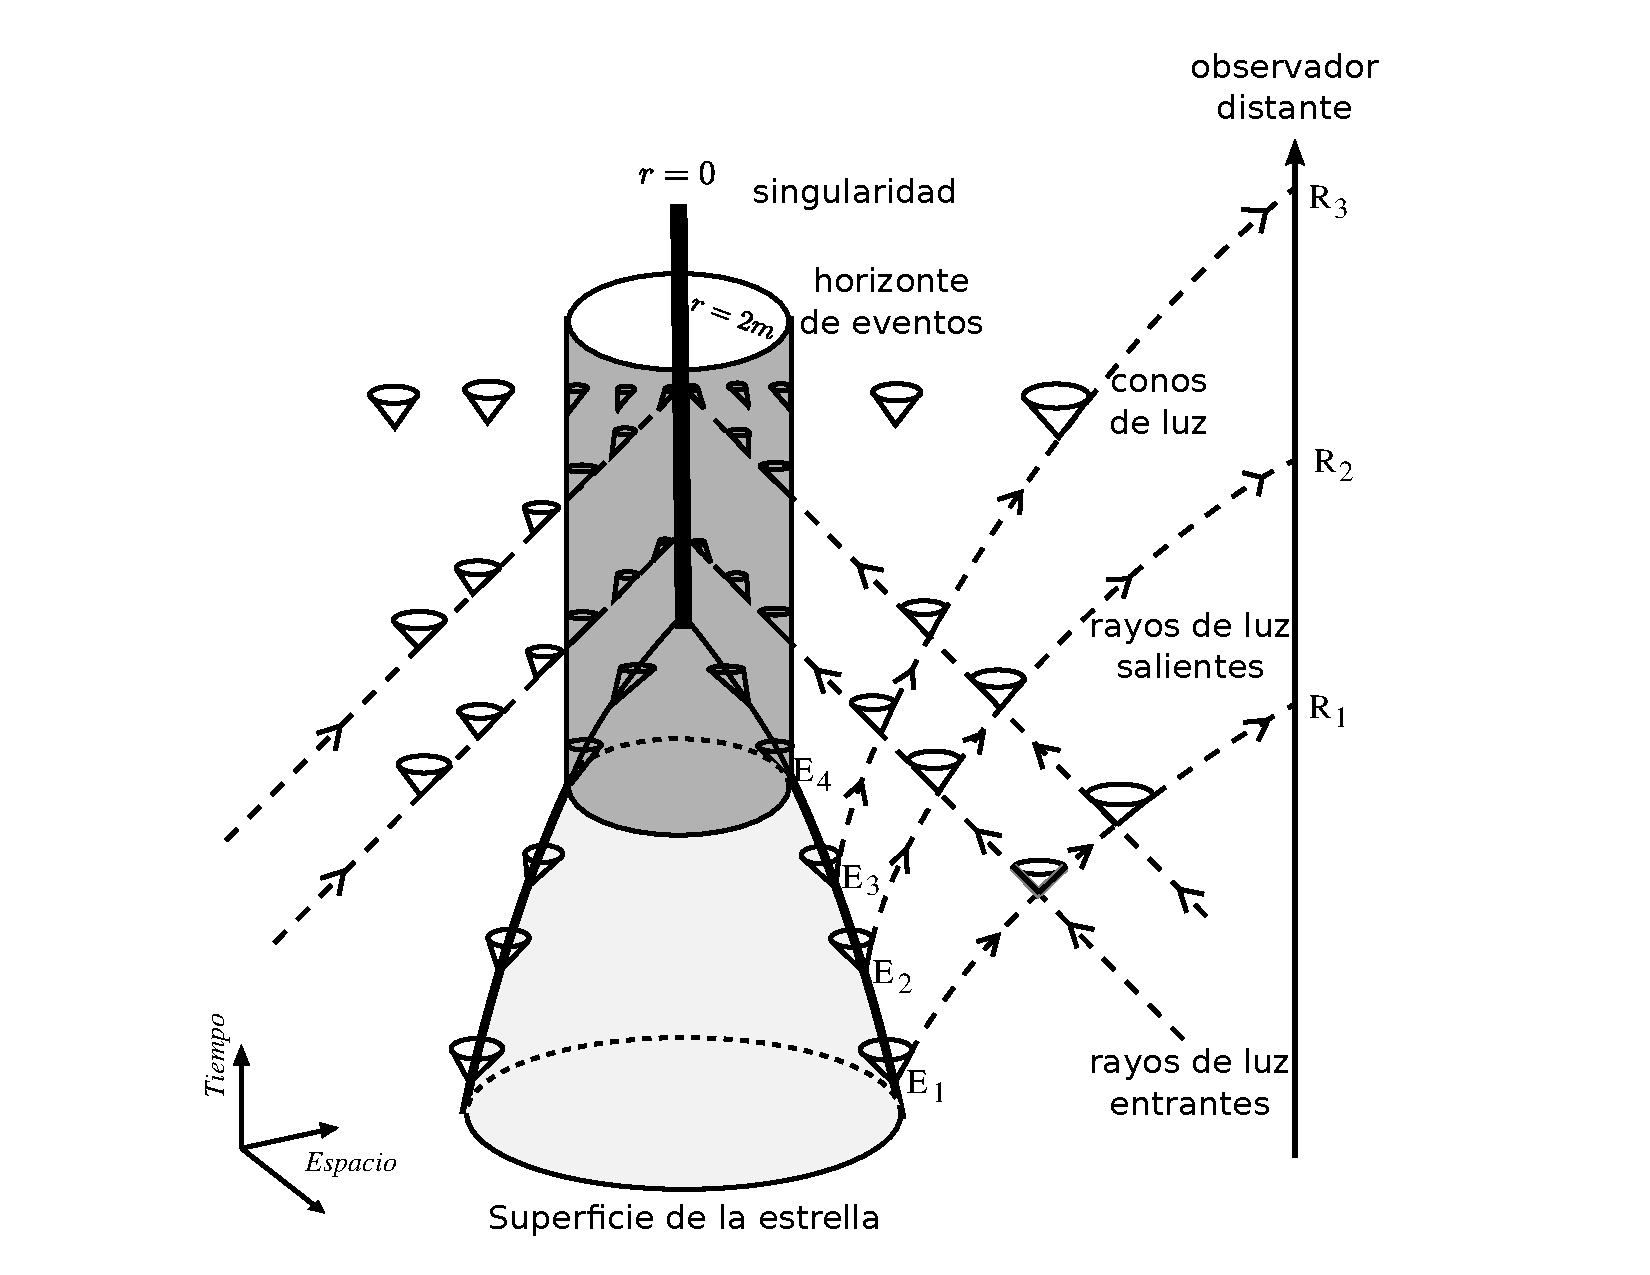
\includegraphics[height=7cm]{fig/fig-colapso.pdf}
\caption{Colapso estelar, figura adaptada a partir de Ref. \cite{Luminet98}}
\label{fig:colapso}
\end{center}
\end{figure}